\documentclass[aspectratio=169,10pt]{beamer}

% ------------------------------------------------------------------------------
% Packages
% ------------------------------------------------------------------------------
\usepackage[T1]{fontenc}
\usepackage[utf8]{inputenc}
\usepackage{lmodern}
\usepackage{booktabs}
\usepackage{array}
\usepackage{amsmath}
\usepackage{graphicx}
\usepackage{tikz}
\usetikzlibrary{arrows.meta, positioning, shapes.geometric, fit, calc, backgrounds}

% ------------------------------------------------------------------------------
% Minimalist Black & White Theme
% ------------------------------------------------------------------------------
\definecolor{bwBlack}{HTML}{000000}
\definecolor{bwCharcoal}{HTML}{1F1F1F}
\definecolor{bwGray}{HTML}{666666}
\definecolor{bwLightGray}{HTML}{E5E5E5}
\definecolor{bwOffWhite}{HTML}{F7F7F7}
\definecolor{bwWhite}{HTML}{FFFFFF}

\setbeamercolor{background canvas}{bg=bwWhite}
\setbeamercolor{normal text}{fg=bwCharcoal,bg=bwWhite}
\setbeamercolor{title}{fg=bwBlack}
\setbeamercolor{subtitle}{fg=bwGray}
\setbeamercolor{author}{fg=bwCharcoal}
\setbeamercolor{date}{fg=bwGray}
\setbeamercolor{frametitle}{fg=bwBlack}
\setbeamercolor{framesubtitle}{fg=bwGray}
\setbeamercolor{structure}{fg=bwBlack}
\setbeamercolor{itemize item}{fg=bwBlack}
\setbeamercolor{itemize subitem}{fg=bwGray}
\setbeamercolor{block title}{fg=bwBlack,bg=bwOffWhite}
\setbeamercolor{block body}{fg=bwCharcoal,bg=bwWhite}

\setbeamerfont{title}{size=\LARGE,series=\bfseries}
\setbeamerfont{subtitle}{size=\normalsize,series=\normalfont}
\setbeamerfont{frametitle}{size=\Large,series=\bfseries}
\setbeamerfont{framesubtitle}{size=\small,series=\normalfont}
\setbeamerfont{footnote}{size=\scriptsize}

\setbeamertemplate{navigation symbols}{}
\setbeamertemplate{itemize items}[square]
\setbeamertemplate{itemize subitem}{--}

\setbeamertemplate{frametitle}{%
  \vspace{0.3em}
  \insertframetitle\par
  \ifx\insertframesubtitle\@empty\else
    {\usebeamerfont{framesubtitle}\usebeamercolor[fg]{framesubtitle}\insertframesubtitle\par}%
  \fi
  \vspace{0.18em}
  {\color{bwBlack}\hrule height 0.6pt}
  \vspace{0.25em}
}

\setbeamertemplate{footline}{%
  \leavevmode%
  \hbox{%
    \begin{beamercolorbox}[wd=.75\paperwidth,ht=2.3ex,dp=1.1ex,leftskip=1.5em]{date}%
      \color{bwGray}\scriptsize StudentFeedback $\cdot$ Multi-Task Sentiment \& Topic Classification
    \end{beamercolorbox}%
    \begin{beamercolorbox}[wd=.25\paperwidth,ht=2.3ex,dp=1.1ex,right,rightskip=1.5em]{date}%
      \color{bwGray}\scriptsize \insertframenumber{} / \inserttotalframenumber
    \end{beamercolorbox}%
  }%
  \vskip0.25em%
}

% ------------------------------------------------------------------------------
% TikZ Styles (Neural Network & Architectural Diagrams, Strict B&W)
% ------------------------------------------------------------------------------
\tikzset{
  tok/.style={
    rectangle,
    draw=bwGray,
    line width=0.5pt,
    fill=bwOffWhite,
    rounded corners=1.5pt,
    minimum width=0.85cm,
    minimum height=0.45cm,
    font=\tiny\ttfamily,
    align=center
  },
  emb/.style={
    rectangle,
    draw=bwBlack,
    line width=0.6pt,
    fill=bwWhite,
    minimum width=0.85cm,
    minimum height=0.45cm,
    font=\tiny\sffamily,
    align=center
  },
  cell/.style={
    rectangle,
    draw=bwBlack,
    line width=0.7pt,
    fill=bwWhite,
    rounded corners=2pt,
    minimum width=0.95cm,
    minimum height=0.52cm,
    font=\tiny\bfseries\sffamily,
    align=center
  },
  cellbwd/.style={
    cell,
    fill=bwOffWhite
  },
  neuron/.style={
    circle,
    draw=bwBlack,
    line width=0.65pt,
    fill=bwWhite,
    minimum size=0.34cm,
    inner sep=0pt
  },
  neurondark/.style={
    neuron,
    fill=bwBlack
  },
  opcircle/.style={
    circle,
    draw=bwBlack,
    line width=0.65pt,
    fill=bwWhite,
    minimum size=0.38cm,
    inner sep=0pt,
    font=\tiny\bfseries
  },
  modbox/.style={
    rectangle,
    draw=bwBlack,
    line width=0.7pt,
    fill=bwWhite,
    rounded corners=2pt,
    align=center,
    font=\scriptsize\sffamily,
    inner sep=4pt
  },
  modboxfill/.style={
    modbox,
    fill=bwOffWhite
  },
  modboxdark/.style={
    modbox,
    fill=bwBlack,
    text=bwWhite
  },
  arr/.style={
    -{Stealth[length=1.6mm,width=1.1mm]},
    draw=bwBlack,
    line width=0.6pt
  },
  arrgray/.style={
    -{Stealth[length=1.4mm,width=1.0mm]},
    draw=bwGray,
    line width=0.5pt
  },
  synapse/.style={
    draw=bwGray,
    line width=0.4pt
  },
  dashedframe/.style={
    rectangle,
    draw=bwGray,
    dashed,
    line width=0.6pt,
    rounded corners=2pt,
    inner sep=5pt
  }
}

% ------------------------------------------------------------------------------
% Metadata
% ------------------------------------------------------------------------------
\title{Student Feedback Analysis}
\subtitle{Multi-Task Sentiment \& Topic Classification with RNN, LSTM, and Transformer}
\author{Repository Technical Overview}
\date{November 2026}

\begin{document}

% ==============================================================================
% SLIDE 1: Title
% ==============================================================================
\begin{frame}[plain]
  \vspace{2.2cm}
  {\color{bwBlack}\hrule height 1.2pt}
  \vspace{0.8cm}
  {\usebeamerfont{title}\usebeamercolor[fg]{title}\inserttitle\par}
  \vspace{0.3cm}
  {\usebeamerfont{subtitle}\usebeamercolor[fg]{subtitle}\insertsubtitle\par}
  \vspace{1.2cm}
  {\color{bwLightGray}\hrule height 0.5pt}
  \vspace{0.4cm}
  {\small\color{bwGray}
    \textbf{Tasks:} Binary Sentiment $\times$ 3-Class Topic \quad$\cdot$\quad
    \textbf{Backbones:} BiGRU, BiLSTM, Transformer Encoder
  }
\end{frame}

% ==============================================================================
% SLIDE 2: Problem Formulation & Dataset Splits
% ==============================================================================
\begin{frame}{Problem Formulation \& Dataset}
  \framesubtitle{Jointly predicting student sentiment and feedback topic from a single text sequence}
  \begin{columns}[T,totalwidth=\textwidth]
    \begin{column}{0.52\textwidth}
      \textbf{Multi-Task Formulation}
      \begin{itemize}
        \item \textbf{Sentiment Classification (2 classes):}\\
              \texttt{negative} (0), \texttt{positive} (1).\\
              {\scriptsize\color{bwGray} Neutral (1) excluded; original label 2 remapped to 1.}
        \item \textbf{Topic Classification (3 classes):}\\
              \texttt{lecturer} (0), \texttt{training\_program} (1), \texttt{facility} (2).\\
              {\scriptsize\color{bwGray} Others (3) excluded to focus on core academic feedback.}
      \end{itemize}

      \vspace{0.4em}
      \textbf{Why Multi-Task Learning?}
      \begin{itemize}\scriptsize
        \item Shared text encoder captures both evaluative tone and domain keywords.
        \item Reduces parameter footprint and inference latency ($1$ forward pass vs. $2$ models).
      \end{itemize}
    \end{column}

    \begin{column}{0.45\textwidth}
      \textbf{Dataset Splits (UIT-VSFC)}
      \vspace{0.3em}
      \begin{table}
        \centering
        \footnotesize
        \begin{tabular}{@{}lrrr@{}}
          \toprule
          \textbf{Split} & \textbf{Raw} & \textbf{Filtered} & \textbf{Kept (\%)} \\
          \midrule
          Train          & 11,426       & 10,567            & 92.5\% \\
          Validation     & 1,583        & 1,441             & 91.0\% \\
          Test           & 3,166        & 2,884             & 91.1\% \\
          \midrule
          \textbf{Total} & \textbf{16,175} & \textbf{14,892} & \textbf{92.1\%} \\
          \bottomrule
        \end{tabular}
      \end{table}

      \vspace{0.4em}
      \textbf{Preprocessing (\texttt{data\_utils.py})}
      \begin{itemize}\scriptsize
        \item Lowercase + whitespace tokenization.
        \item Vocabulary built from \texttt{train} only (\texttt{min\_freq=2}).
      \end{itemize}
    \end{column}
  \end{columns}
\end{frame}

% ==============================================================================
% SLIDE 3: Dataset Analysis - Sentiment Distribution
% ==============================================================================
\begin{frame}{Dataset Analysis: Sentiment Distribution}
  \framesubtitle{Balanced binary classes across Train, Validation, and Test splits}
  \begin{columns}[c,totalwidth=\textwidth]
    \begin{column}{0.64\textwidth}
      \centering
      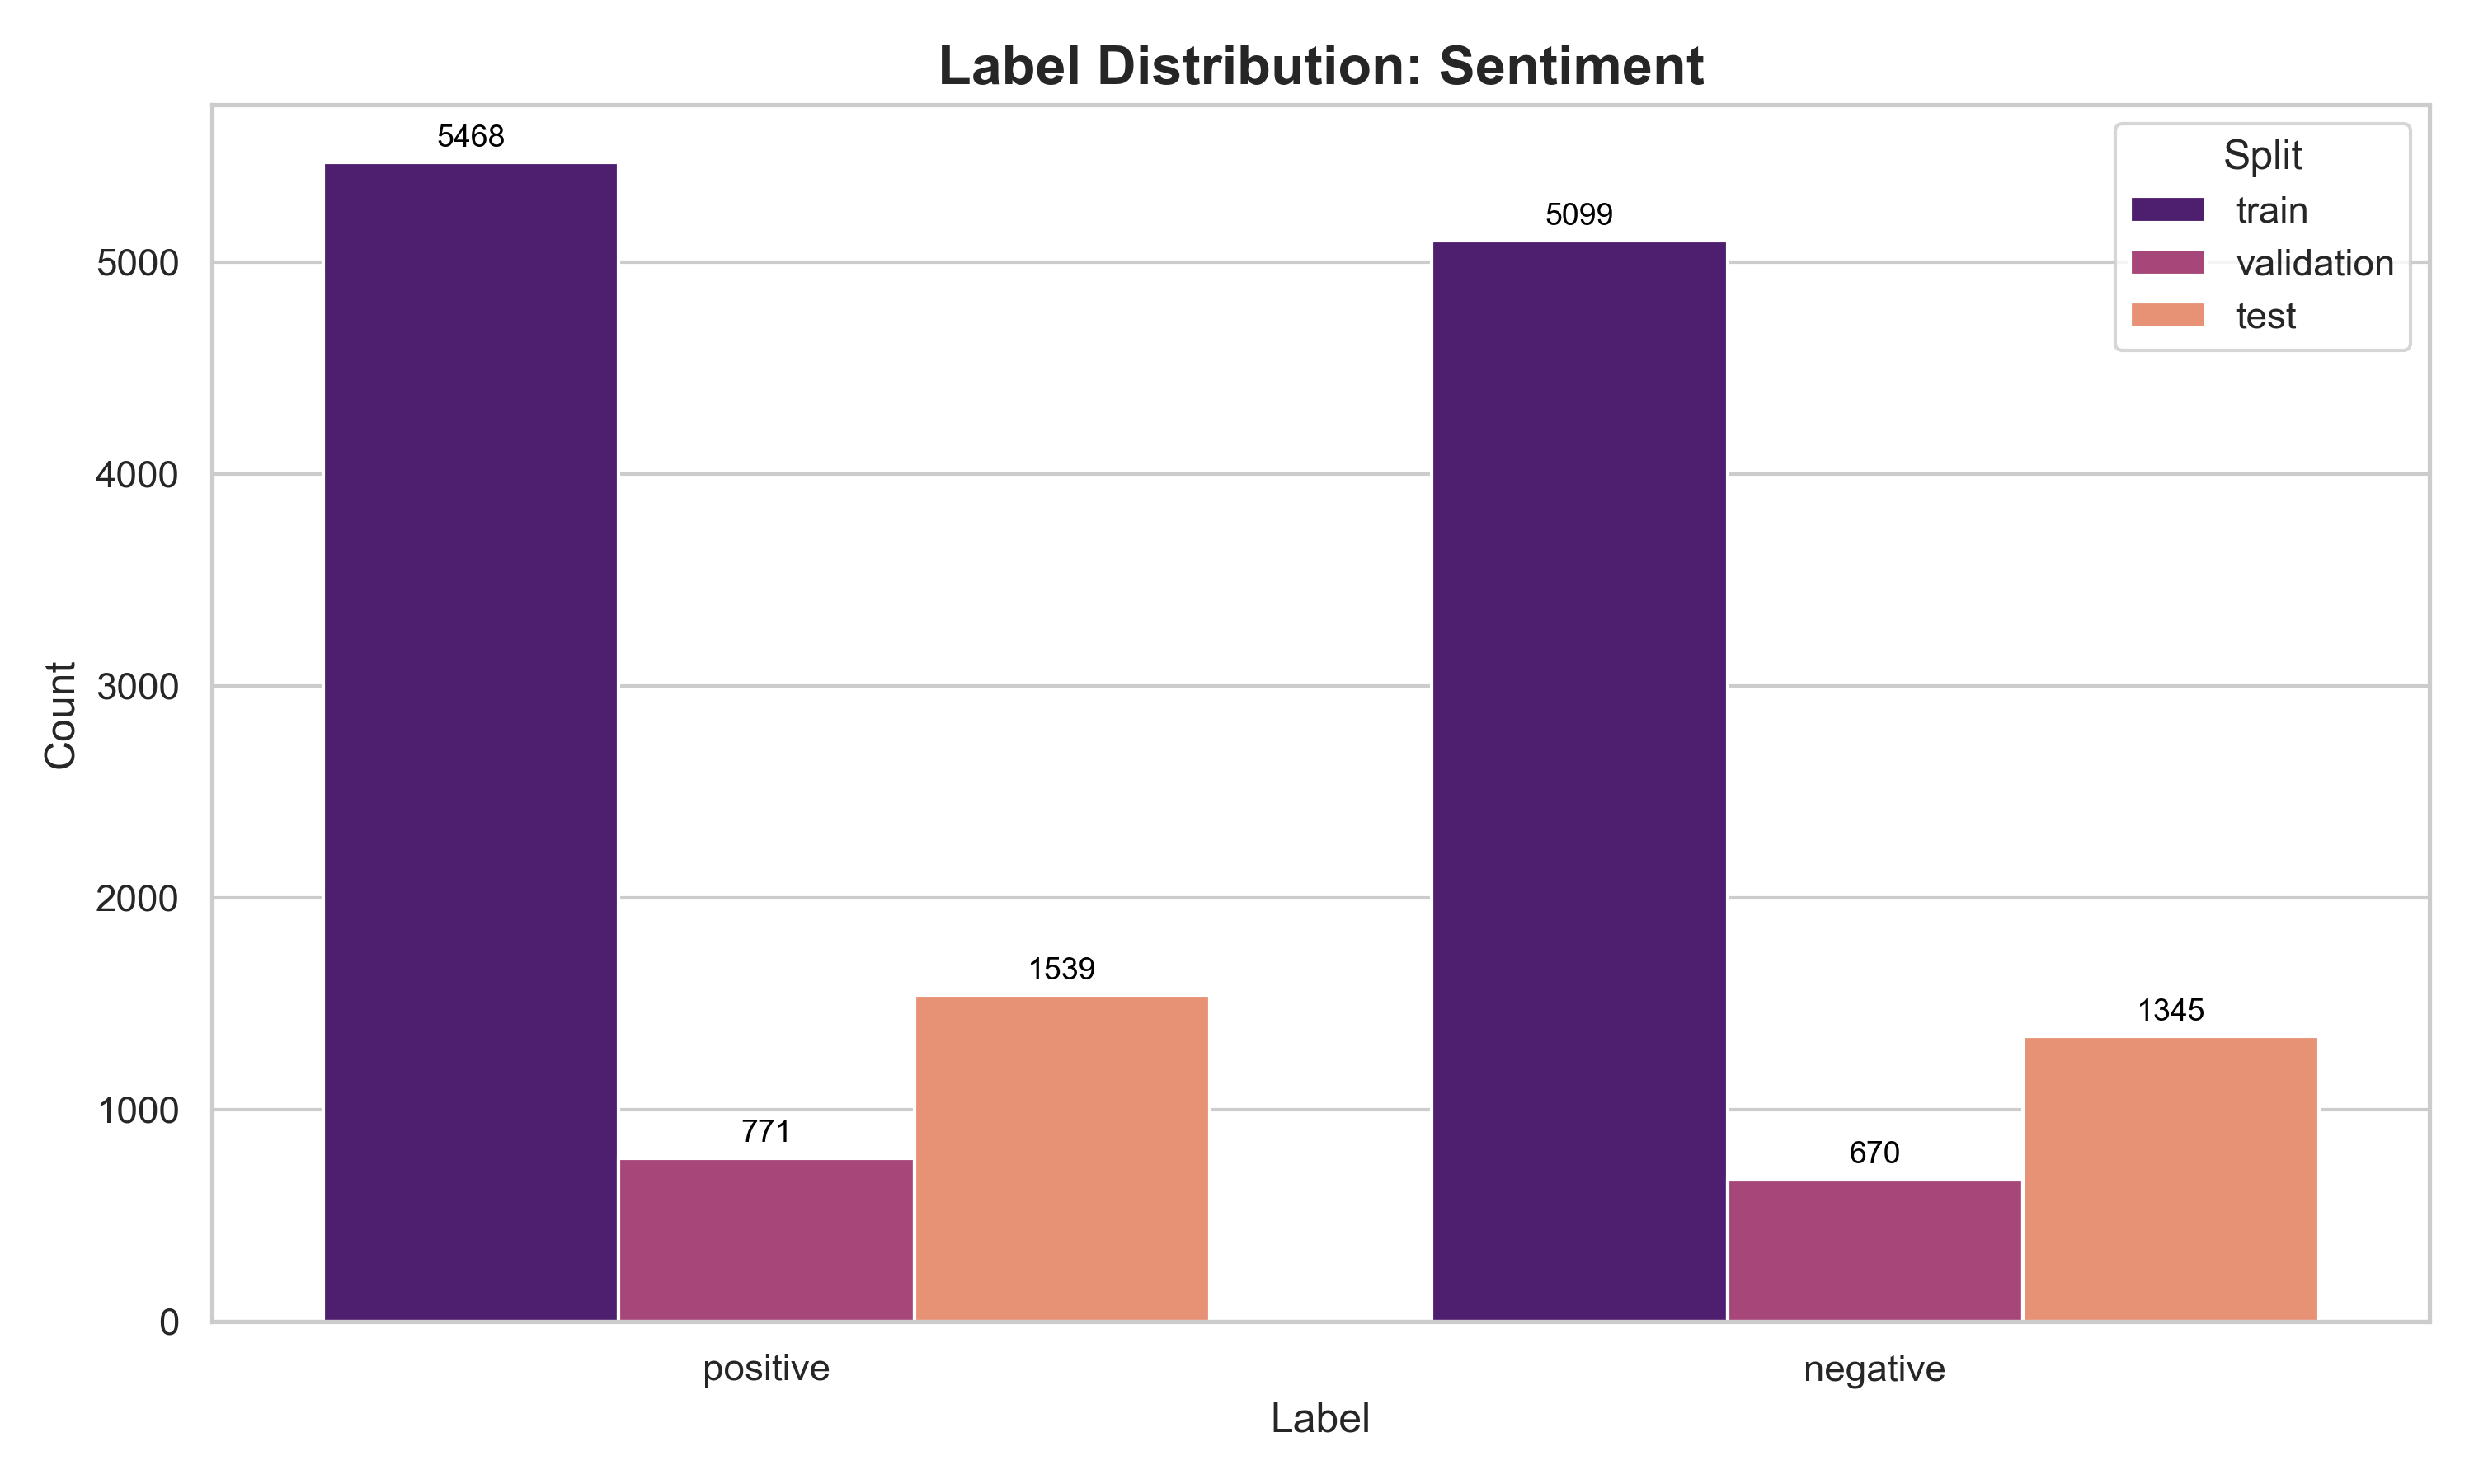
\includegraphics[width=\linewidth,height=0.78\textheight,keepaspectratio]{../images/sentiment_distribution.png}
    \end{column}
    \begin{column}{0.34\textwidth}
      \textbf{Distribution Analysis}
      \begin{itemize}
        \item \textbf{Near-balanced split:} Both \texttt{negative} and \texttt{positive} are well represented across all three splits.
        \item \textbf{Test support ($N=2,884$):}
              \begin{itemize}\scriptsize
                \item \texttt{negative}: 1,345 (46.6\%)
                \item \texttt{positive}: 1,539 (53.4\%)
              \end{itemize}
        \item \textbf{Implication:} Standard Cross-Entropy with mild label smoothing ($\alpha=0.1$) is sufficient without class re-weighting.
      \end{itemize}
    \end{column}
  \end{columns}
\end{frame}

% ==============================================================================
% SLIDE 4: Dataset Analysis - Topic Distribution
% ==============================================================================
\begin{frame}{Dataset Analysis: Topic Distribution}
  \framesubtitle{Strong class imbalance dominated by \texttt{lecturer} feedback}
  \begin{columns}[c,totalwidth=\textwidth]
    \begin{column}{0.64\textwidth}
      \centering
      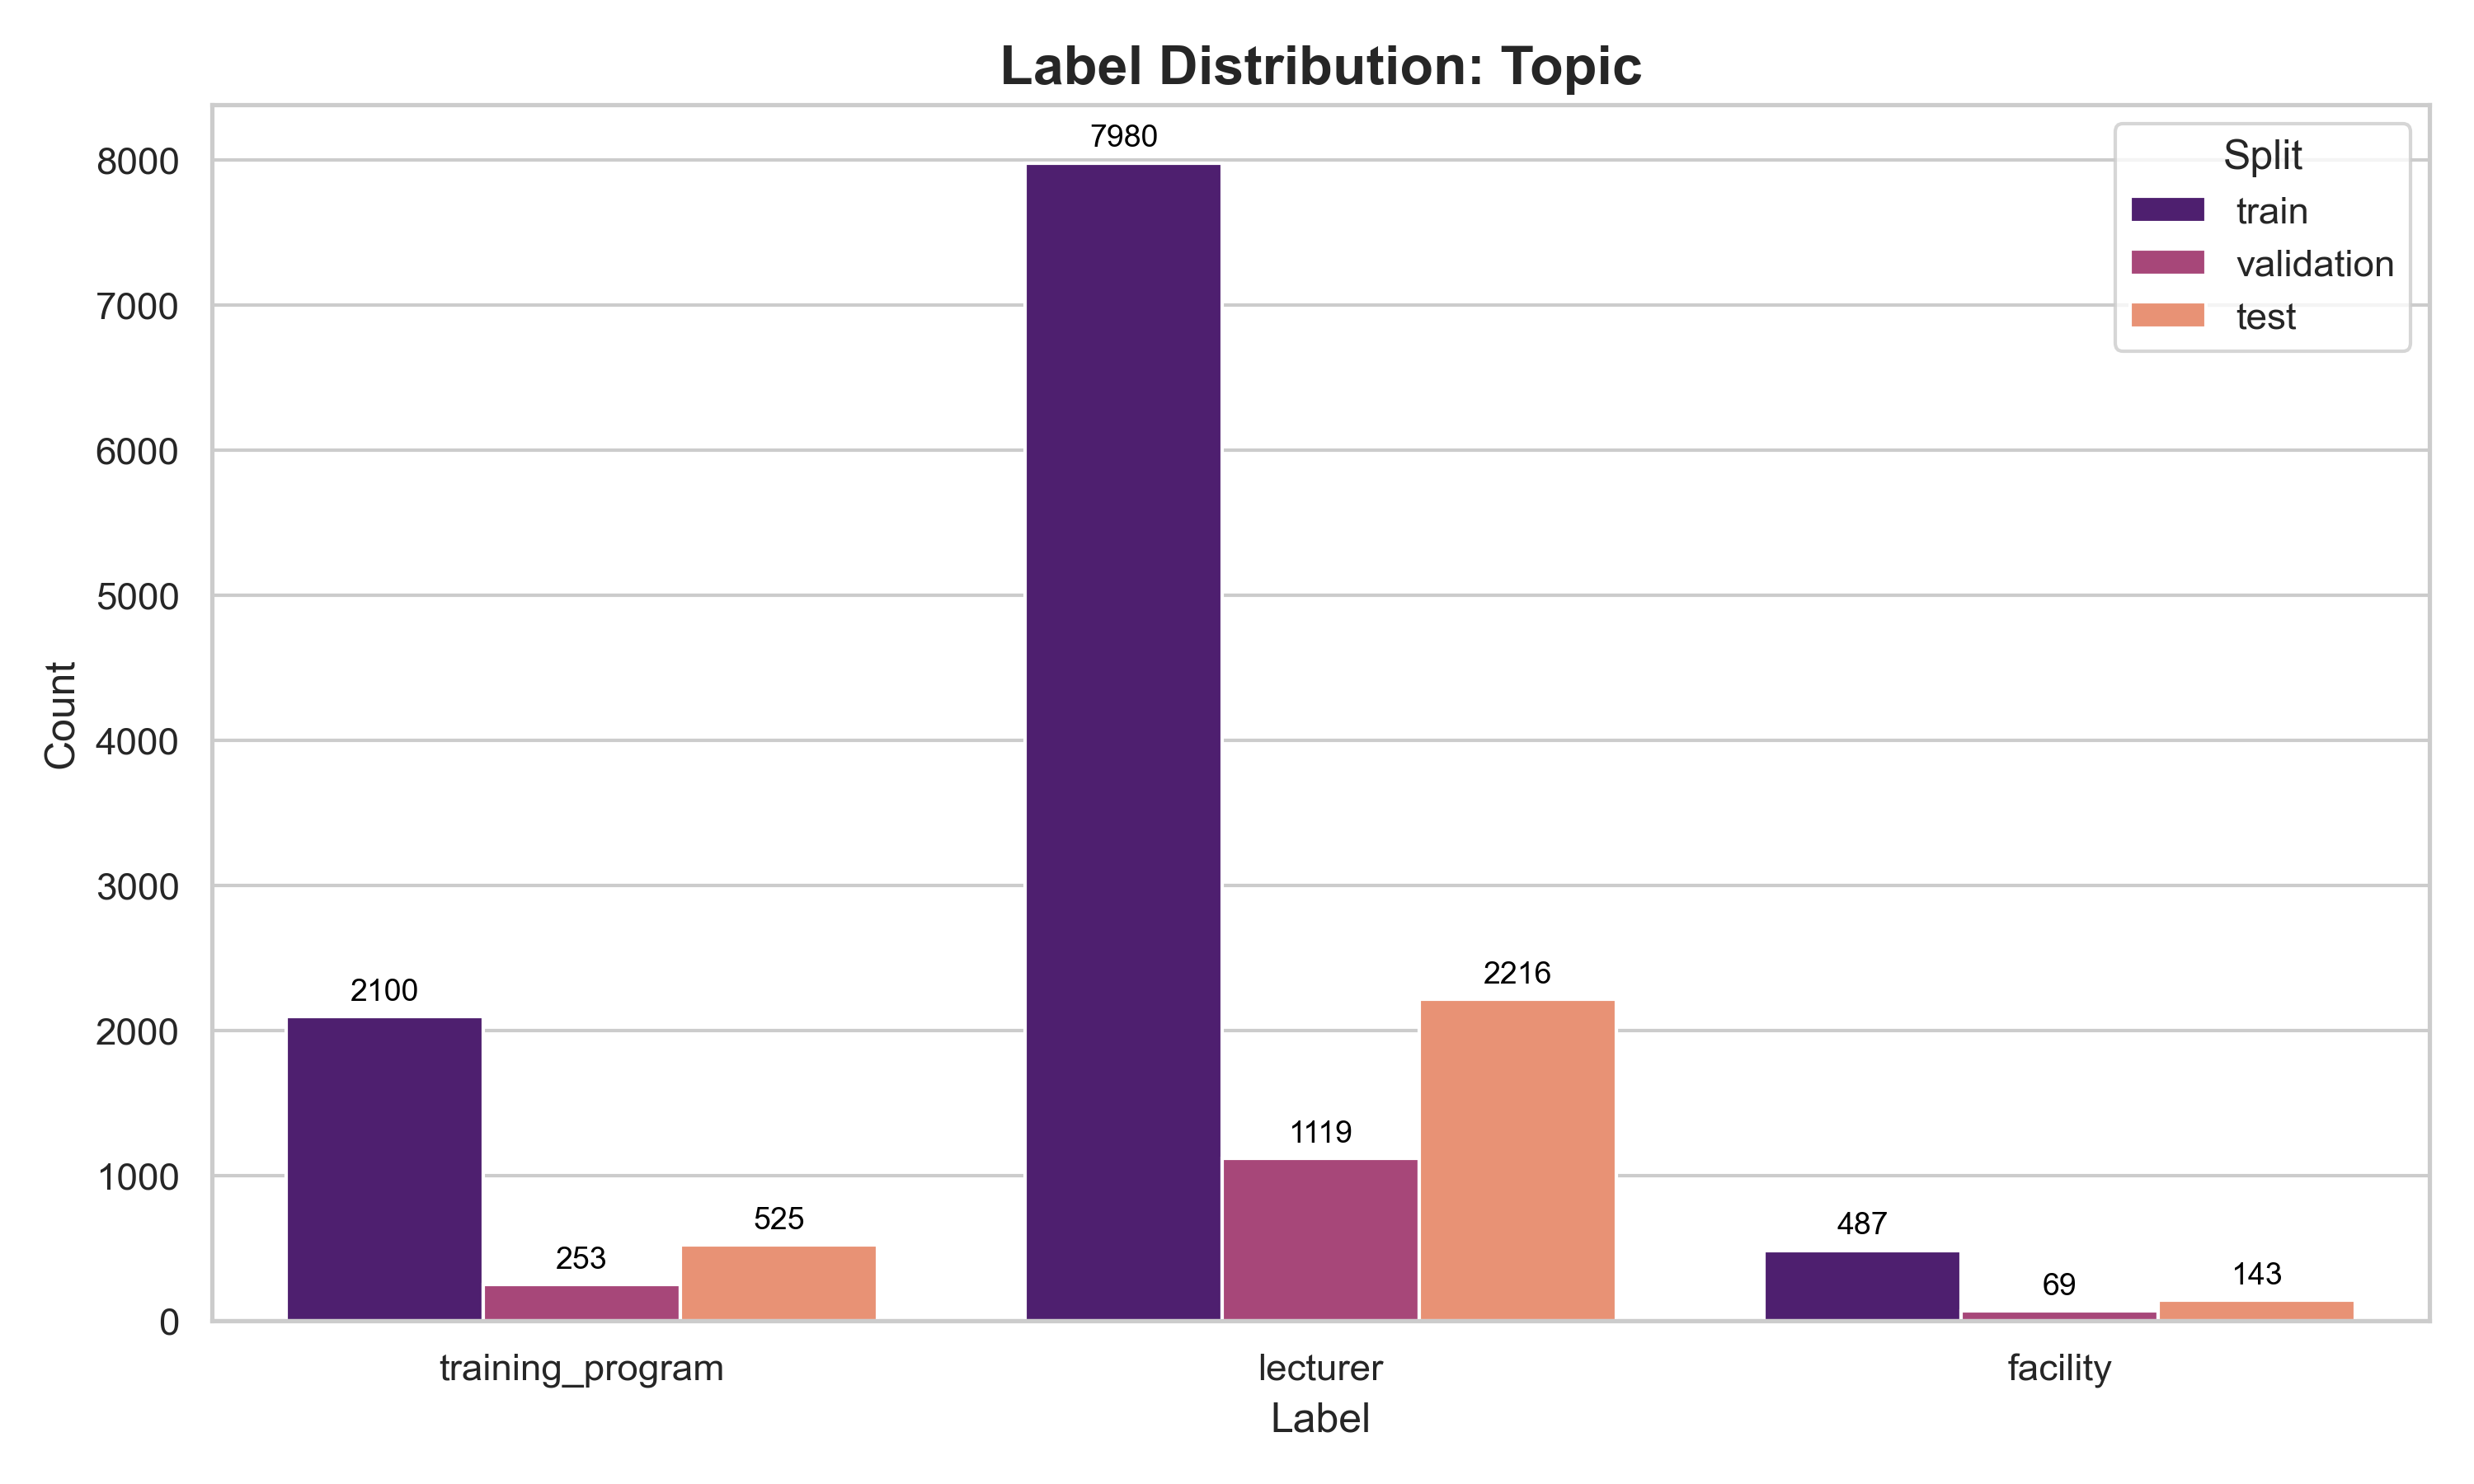
\includegraphics[width=\linewidth,height=0.78\textheight,keepaspectratio]{../images/topic_distribution.png}
    \end{column}
    \begin{column}{0.34\textwidth}
      \textbf{Imbalance Analysis}
      \begin{itemize}
        \item \textbf{Test support ($N=2,884$):}
              \begin{itemize}\scriptsize
                \item \texttt{lecturer}: 2,216 (76.8\%)
                \item \texttt{training\_program}: 525 (18.2\%)
                \item \texttt{facility}: 143 (5.0\%)
              \end{itemize}
        \item \textbf{Key challenge:} \texttt{facility} has distinct keywords (room, projector, wifi), whereas \texttt{training\_program} often overlaps lexically with \texttt{lecturer}.
        \item \textbf{Mitigation:} Higher label smoothing ($\alpha=0.2$) and Macro-F1 tracking.
      \end{itemize}
    \end{column}
  \end{columns}
\end{frame}

% ==============================================================================
% SLIDE 5: Repository & Pipeline Architecture
% ==============================================================================
\begin{frame}{Repository \& Training Pipeline}
  \framesubtitle{CLI-driven workflow (\texttt{run.py}) backed by \texttt{config.yml} and Weights \& Biases}
  \centering
  \vspace{0.15cm}
  \resizebox{0.96\textwidth}{!}{%
  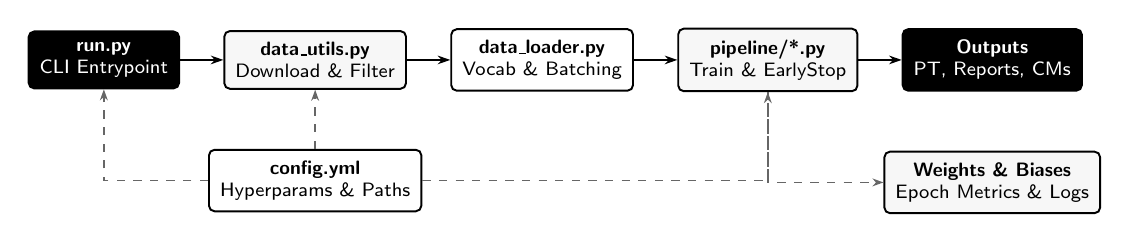
\begin{tikzpicture}[node distance=0.45cm and 0.55cm]
    \node[modboxdark] (cli) {\textbf{run.py}\\CLI Entrypoint};
    \node[modboxfill, right=of cli] (data) {\textbf{data\_utils.py}\\Download \& Filter};
    \node[modbox, right=of data] (loader) {\textbf{data\_loader.py}\\Vocab \& Batching};
    \node[modboxfill, right=of loader] (train) {\textbf{pipeline/*.py}\\Train \& EarlyStop};
    \node[modboxdark, right=of train] (eval) {\textbf{Outputs}\\PT, Reports, CMs};

    \draw[arr] (cli) -- (data);
    \draw[arr] (data) -- (loader);
    \draw[arr] (loader) -- (train);
    \draw[arr] (train) -- (eval);

    \node[modbox, below=0.75cm of data] (cfg) {\textbf{config.yml}\\Hyperparams \& Paths};
    \node[modboxfill, below=0.75cm of eval] (wb) {\textbf{Weights \& Biases}\\Epoch Metrics \& Logs};
    \draw[arrgray, dashed] (cfg) -| (cli);
    \draw[arrgray, dashed] (cfg) -- (data);
    \draw[arrgray, dashed] (cfg) -| (train);
    \draw[arrgray, dashed] (train) |- (wb);
  \end{tikzpicture}%
  }

  \vspace{0.45cm}
  \begin{columns}[T,totalwidth=\textwidth]
    \begin{column}{0.32\textwidth}
      \textbf{1. CLI Tasks (\texttt{run.py})}
      \begin{itemize}\scriptsize
        \item \texttt{-{}-task download}: Fetch 9 splits via \texttt{gdown}
        \item \texttt{-{}-task data-vis}: Plot label distributions
        \item \texttt{-{}-task pipeline -{}-model ...}: Train + eval
      \end{itemize}
    \end{column}
    \begin{column}{0.32\textwidth}
      \textbf{2. Batching \& Reproducibility}
      \begin{itemize}\scriptsize
        \item Dynamic batch padding (\texttt{pad\_sequence})
        \item Emits \texttt{input\_ids}, \texttt{lengths}, \texttt{attention\_mask}
        \item Global seed \texttt{42}, deterministic ops enabled
      \end{itemize}
    \end{column}
    \begin{column}{0.32\textwidth}
      \textbf{3. Experiment Tracking}
      \begin{itemize}\scriptsize
        \item Logs train/val loss, acc, macro-F1, LR per epoch
        \item Saves best checkpoint via \texttt{EarlyStopping}
        \item Exports classification reports \& confusion matrices
      \end{itemize}
    \end{column}
  \end{columns}
\end{frame}

% ==============================================================================
% SLIDE 6: Model 1 - BidirLSTM Neural Architecture
% ==============================================================================
\begin{frame}{Model 1: \texttt{BidirLSTM} Neural Architecture}
  \framesubtitle{2-layer Bidirectional LSTM over packed embeddings with dual linear classification heads}
  \begin{columns}[c,totalwidth=\textwidth]
    \begin{column}{0.64\textwidth}
      \centering
      \resizebox{\linewidth}{!}{%
      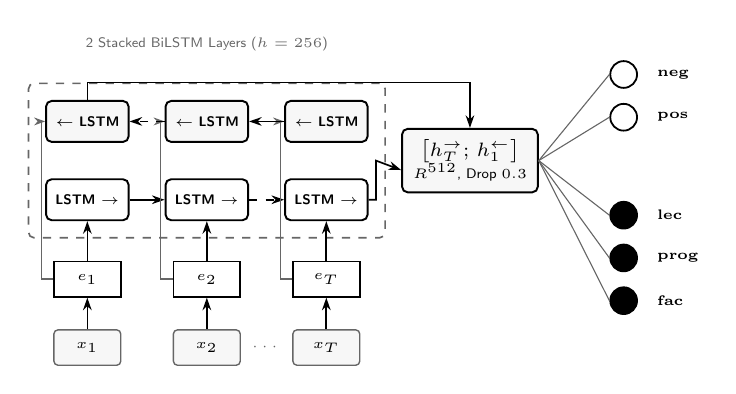
\begin{tikzpicture}[node distance=0.35cm and 0.45cm]
        % Tokens
        \node[tok] (x1) {$x_1$};
        \node[tok, right=0.65cm of x1] (x2) {$x_2$};
        \node[tok, right=0.65cm of x2] (xt) {$x_T$};
        \node[font=\tiny, color=bwGray] at ($(x2)!0.5!(xt)$) {$\cdots$};

        % Embeddings
        \node[emb, above=0.40cm of x1] (e1) {$e_1$};
        \node[emb, above=0.40cm of x2] (e2) {$e_2$};
        \node[emb, above=0.40cm of xt] (et) {$e_T$};
        \draw[arr] (x1) -- (e1);
        \draw[arr] (x2) -- (e2);
        \draw[arr] (xt) -- (et);

        % Forward LSTM Layer
        \node[cell, above=0.50cm of e1] (f1) {LSTM $\rightarrow$};
        \node[cell, above=0.50cm of e2] (f2) {LSTM $\rightarrow$};
        \node[cell, above=0.50cm of et] (ft) {LSTM $\rightarrow$};
        \draw[arr] (e1) -- (f1);
        \draw[arr] (e2) -- (f2);
        \draw[arr] (et) -- (ft);
        \draw[arr] (f1) -- (f2);
        \draw[arr, dashed] (f2) -- (ft);

        % Backward LSTM Layer
        \node[cellbwd, above=0.45cm of f1] (b1) {$\leftarrow$ LSTM};
        \node[cellbwd, above=0.45cm of f2] (b2) {$\leftarrow$ LSTM};
        \node[cellbwd, above=0.45cm of ft] (bt) {$\leftarrow$ LSTM};
        \draw[arrgray] (e1.west) -- ++(-0.15,0) |- (b1.west);
        \draw[arrgray] (e2.west) -- ++(-0.15,0) |- (b2.west);
        \draw[arrgray] (et.west) -- ++(-0.15,0) |- (bt.west);
        \draw[arr] (bt) -- (b2);
        \draw[arr, dashed] (b2) -- (b1);

        \begin{scope}[on background layer]
          \node[dashedframe, fit=(f1)(bt), inner sep=6pt, label={[font=\tiny\sffamily,color=bwGray,yshift=0.28cm]above:2 Stacked BiLSTM Layers ($h=256$)}] (encframe) {};
        \end{scope}

        % Concatenation & Dropout (cleanly outside encframe)
        \node[modboxfill, right=0.95cm of $(ft)!0.5!(bt)$, minimum width=1.45cm] (cat) {$\big[h_T^{\rightarrow};\, h_1^{\leftarrow}\big]$\\{\tiny $\mathbb{R}^{512}$, Drop $0.3$}};
        \draw[arr] (ft.east) -| ($(cat.west)+(-0.32,0)$) -- ($(cat.west)+(0,-0.12)$);
        \draw[arr] (b1.north) -- ++(0,0.22) -| ($(cat.north)$);

        % Neural Head Neurons: Sentiment (2) & Topic (3)
        \node[neuron, above right=0.55cm and 0.95cm of cat] (s1) {};
        \node[neuron, below=0.18cm of s1] (s2) {};
        \node[font=\tiny\bfseries, right=0.12cm of s1] {neg};
        \node[font=\tiny\bfseries, right=0.12cm of s2] {pos};

        \node[neurondark, below right=0.15cm and 0.95cm of cat] (t1) {};
        \node[neurondark, below=0.18cm of t1] (t2) {};
        \node[neurondark, below=0.18cm of t2] (t3) {};
        \node[font=\tiny\bfseries, right=0.12cm of t1] {lec};
        \node[font=\tiny\bfseries, right=0.12cm of t2] {prog};
        \node[font=\tiny\bfseries, right=0.12cm of t3] {fac};

        \foreach \n in {s1,s2,t1,t2,t3} {
          \draw[synapse] (cat.east) -- (\n.west);
        }
      \end{tikzpicture}%
      }
    \end{column}

    \begin{column}{0.34\textwidth}
      \textbf{Architecture Specs}
      \begin{itemize}\scriptsize
        \item \textbf{Embedding:} $V \times 300$, \texttt{dropout=0.3}
        \item \textbf{Encoder:} 2-layer BiLSTM, $h=256$ per direction
        \item \textbf{Packed seq:} Ignores \texttt{<pad>} tokens
        \item \textbf{Shared state:} $512$-dim vector
        \item \textbf{Heads:} Linear $512 \to 2$ \& $512 \to 3$
      \end{itemize}
      \vspace{0.3em}
      \textbf{Training Config}
      \begin{itemize}\scriptsize
        \item AdamW: $\text{lr}=10^{-3}$, $\text{wd}=10^{-3}$
        \item Batch size: $64$, Epochs: $50$ (patience $10$)
        \item Checkpoint size: \textbf{12.66 MB}
      \end{itemize}
    \end{column}
  \end{columns}
\end{frame}

% ==============================================================================
% SLIDE 7: Model 2 - BidirRNN (BiGRU) Neural Architecture
% ==============================================================================
\begin{frame}{Model 2: \texttt{BidirRNN} (BiGRU) Neural Architecture}
  \framesubtitle{Compact 2-layer Bidirectional GRU with gradient clipping and LR plateau scheduling}
  \begin{columns}[c,totalwidth=\textwidth]
    \begin{column}{0.64\textwidth}
      \centering
      \resizebox{\linewidth}{!}{%
      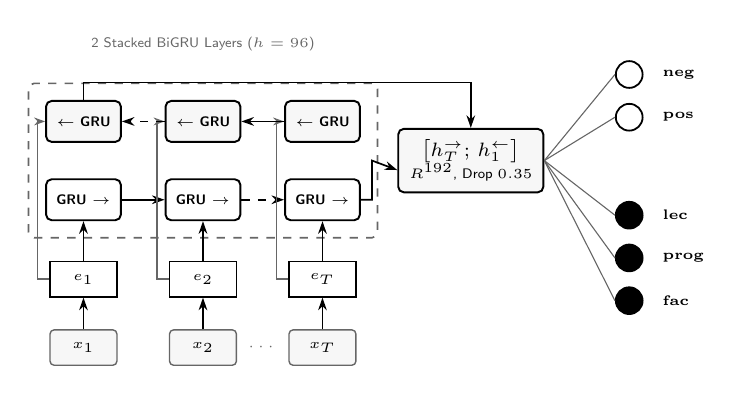
\begin{tikzpicture}[node distance=0.35cm and 0.45cm]
        \node[tok] (x1) {$x_1$};
        \node[tok, right=0.65cm of x1] (x2) {$x_2$};
        \node[tok, right=0.65cm of x2] (xt) {$x_T$};
        \node[font=\tiny, color=bwGray] at ($(x2)!0.5!(xt)$) {$\cdots$};

        \node[emb, above=0.40cm of x1] (e1) {$e_1$};
        \node[emb, above=0.40cm of x2] (e2) {$e_2$};
        \node[emb, above=0.40cm of xt] (et) {$e_T$};
        \draw[arr] (x1) -- (e1);
        \draw[arr] (x2) -- (e2);
        \draw[arr] (xt) -- (et);

        \node[cell, above=0.50cm of e1] (f1) {GRU $\rightarrow$};
        \node[cell, above=0.50cm of e2] (f2) {GRU $\rightarrow$};
        \node[cell, above=0.50cm of et] (ft) {GRU $\rightarrow$};
        \draw[arr] (e1) -- (f1);
        \draw[arr] (e2) -- (f2);
        \draw[arr] (et) -- (ft);
        \draw[arr] (f1) -- (f2);
        \draw[arr, dashed] (f2) -- (ft);

        \node[cellbwd, above=0.45cm of f1] (b1) {$\leftarrow$ GRU};
        \node[cellbwd, above=0.45cm of f2] (b2) {$\leftarrow$ GRU};
        \node[cellbwd, above=0.45cm of ft] (bt) {$\leftarrow$ GRU};
        \draw[arrgray] (e1.west) -- ++(-0.15,0) |- (b1.west);
        \draw[arrgray] (e2.west) -- ++(-0.15,0) |- (b2.west);
        \draw[arrgray] (et.west) -- ++(-0.15,0) |- (bt.west);
        \draw[arr] (bt) -- (b2);
        \draw[arr, dashed] (b2) -- (b1);

        \begin{scope}[on background layer]
          \node[dashedframe, fit=(f1)(bt), inner sep=6pt, label={[font=\tiny\sffamily,color=bwGray,yshift=0.28cm]above:2 Stacked BiGRU Layers ($h=96$)}] (encframe) {};
        \end{scope}

        \node[modboxfill, right=0.95cm of $(ft)!0.5!(bt)$, minimum width=1.45cm] (cat) {$\big[h_T^{\rightarrow};\, h_1^{\leftarrow}\big]$\\{\tiny $\mathbb{R}^{192}$, Drop $0.35$}};
        \draw[arr] (ft.east) -| ($(cat.west)+(-0.32,0)$) -- ($(cat.west)+(0,-0.12)$);
        \draw[arr] (b1.north) -- ++(0,0.22) -| ($(cat.north)$);

        \node[neuron, above right=0.55cm and 0.95cm of cat] (s1) {};
        \node[neuron, below=0.18cm of s1] (s2) {};
        \node[font=\tiny\bfseries, right=0.12cm of s1] {neg};
        \node[font=\tiny\bfseries, right=0.12cm of s2] {pos};

        \node[neurondark, below right=0.15cm and 0.95cm of cat] (t1) {};
        \node[neurondark, below=0.18cm of t1] (t2) {};
        \node[neurondark, below=0.18cm of t2] (t3) {};
        \node[font=\tiny\bfseries, right=0.12cm of t1] {lec};
        \node[font=\tiny\bfseries, right=0.12cm of t2] {prog};
        \node[font=\tiny\bfseries, right=0.12cm of t3] {fac};

        \foreach \n in {s1,s2,t1,t2,t3} {
          \draw[synapse] (cat.east) -- (\n.west);
        }
      \end{tikzpicture}%
      }
    \end{column}

    \begin{column}{0.34\textwidth}
      \textbf{Architecture Specs}
      \begin{itemize}\scriptsize
        \item \textbf{Embedding:} $V \times 128$, \texttt{dropout=0.35}
        \item \textbf{Encoder:} 2-layer BiGRU, $h=96$ per direction
        \item \textbf{Shared state:} $192$-dim vector ($2.7\times$ smaller than BiLSTM)
        \item \textbf{Heads:} Linear $192 \to 2$ \& $192 \to 3$
      \end{itemize}
      \vspace{0.3em}
      \textbf{Training Config}
      \begin{itemize}\scriptsize
        \item AdamW: $\text{lr}=5\times10^{-4}$, $\text{wd}=10^{-4}$
        \item Grad clip $1.0$ + \texttt{ReduceLROnPlateau}
        \item Batch size: $32$, Epochs: $30$ (patience $5$)
        \item Checkpoint size: \textbf{1.95 MB}
      \end{itemize}
    \end{column}
  \end{columns}
\end{frame}

% ==============================================================================
% SLIDE 8: Model 3 - MultiTaskTransformer Neural Architecture
% ==============================================================================
\begin{frame}{Model 3: \texttt{MultiTaskTransformer} Neural Architecture}
  \framesubtitle{2-layer Self-Attention Encoder with learnable positional embeddings and masked mean pooling}
  \begin{columns}[c,totalwidth=\textwidth]
    \begin{column}{0.64\textwidth}
      \centering
      \resizebox{\linewidth}{!}{%
      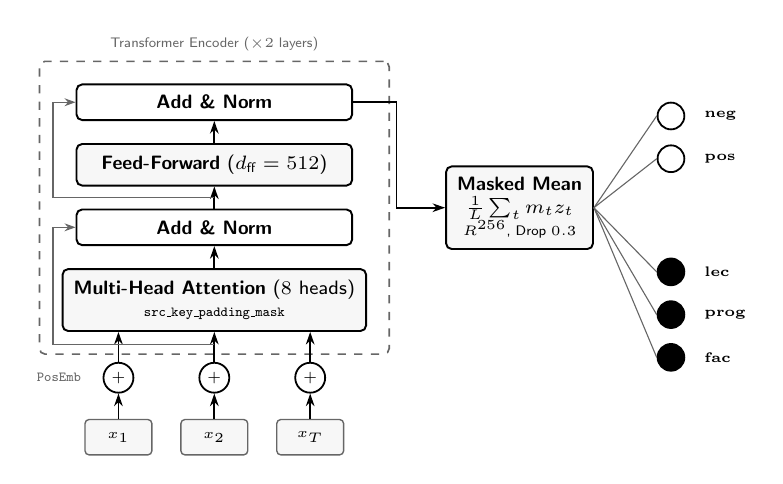
\begin{tikzpicture}[node distance=0.28cm and 0.40cm]
        % Tokens
        \node[tok] (x1) {$x_1$};
        \node[tok, right=0.35cm of x1] (x2) {$x_2$};
        \node[tok, right=0.35cm of x2] (xt) {$x_T$};

        % Token + Pos Emb
        \node[opcircle, above=0.32cm of x1] (p1) {$+$};
        \node[opcircle, above=0.32cm of x2] (p2) {$+$};
        \node[opcircle, above=0.32cm of xt] (pt) {$+$};
        \draw[arr] (x1) -- (p1);
        \draw[arr] (x2) -- (p2);
        \draw[arr] (xt) -- (pt);
        \node[font=\tiny\ttfamily, color=bwGray, left=0.15cm of p1] {PosEmb};

        % Vaswani Encoder Block (bottom to top)
        \node[modboxfill, above=0.38cm of p2, minimum width=3.5cm, minimum height=0.50cm] (mha) {\textbf{Multi-Head Attention} ($8$ heads)\\{\tiny \texttt{src\_key\_padding\_mask}}};
        \draw[arr] (p1.north) -- (p1.north |- mha.south);
        \draw[arr] (p2.north) -- (mha.south);
        \draw[arr] (pt.north) -- (pt.north |- mha.south);

        \node[modbox, above=0.28cm of mha, minimum width=3.5cm, minimum height=0.36cm] (an1) {\textbf{Add \& Norm}};
        \draw[arr] (mha) -- (an1);
        % Residual skip 1
        \coordinate (r1in) at ($(mha.south)+(0,-0.16)$);
        \draw[arrgray] (r1in) -- ++(-2.05,0) |- (an1.west);

        \node[modboxfill, above=0.28cm of an1, minimum width=3.5cm, minimum height=0.40cm] (ffn) {\textbf{Feed-Forward} ($d_{\text{ff}}=512$)};
        \draw[arr] (an1) -- (ffn);

        \node[modbox, above=0.28cm of ffn, minimum width=3.5cm, minimum height=0.36cm] (an2) {\textbf{Add \& Norm}};
        \draw[arr] (ffn) -- (an2);
        % Residual skip 2
        \coordinate (r2in) at ($(an1.north)+(0,0.14)$);
        \draw[arrgray] (r2in) -- ++(-2.05,0) |- (an2.west);

        \begin{scope}[on background layer]
          \node[dashedframe, fit=(mha)(an2), inner sep=8pt, label={[font=\tiny\sffamily,color=bwGray]above:Transformer Encoder ($\times 2$ layers)}] (tframe) {};
        \end{scope}

        % Masked Mean Pooling (cleanly to the right of tframe)
        \node[modboxfill, right=0.70cm of tframe.east, minimum width=1.45cm] (pool) {\textbf{Masked Mean}\\$\frac{1}{L}\sum_{t} m_t z_t$\\{\tiny $\mathbb{R}^{256}$, Drop $0.3$}};
        \draw[arr] (an2.east) -- ++(0.55,0) |- (pool.west);

        % Output Neurons
        \node[neuron, above right=0.50cm and 0.85cm of pool] (s1) {};
        \node[neuron, below=0.18cm of s1] (s2) {};
        \node[font=\tiny\bfseries, right=0.12cm of s1] {neg};
        \node[font=\tiny\bfseries, right=0.12cm of s2] {pos};

        \node[neurondark, below right=0.15cm and 0.85cm of pool] (t1) {};
        \node[neurondark, below=0.18cm of t1] (t2) {};
        \node[neurondark, below=0.18cm of t2] (t3) {};
        \node[font=\tiny\bfseries, right=0.12cm of t1] {lec};
        \node[font=\tiny\bfseries, right=0.12cm of t2] {prog};
        \node[font=\tiny\bfseries, right=0.12cm of t3] {fac};

        \foreach \n in {s1,s2,t1,t2,t3} {
          \draw[synapse] (pool.east) -- (\n.west);
        }
      \end{tikzpicture}%
      }
    \end{column}

    \begin{column}{0.34\textwidth}
      \textbf{Architecture Specs}
      \begin{itemize}\scriptsize
        \item \textbf{Embeddings:} Token ($256$) + Pos ($L_{\max}=512$)
        \item \textbf{Encoder:} 2 blocks, $8$ heads, $\text{FFN}=512$
        \item \textbf{Pooling:} Masked mean over valid tokens
        \item \textbf{Heads:} Linear $256 \to 2$ \& $256 \to 3$
      \end{itemize}
      \vspace{0.3em}
      \textbf{Training Config}
      \begin{itemize}\scriptsize
        \item AdamW: $\text{lr}=10^{-3}$, $\text{wd}=0.0$
        \item Grad clip $1.0$ + \texttt{ReduceLROnPlateau}
        \item Batch size: $64$, Epochs: $50$ (patience $10$)
        \item Checkpoint size: \textbf{6.27 MB}
      \end{itemize}
    \end{column}
  \end{columns}
\end{frame}

% ==============================================================================
% SLIDE 9: Multi-Task Loss & Hyperparameter Comparison
% ==============================================================================
\begin{frame}{Multi-Task Loss \& Training Comparison}
  \framesubtitle{Unified loss weighting across all three architectures}
  \begin{block}{Joint Objective Function}
    \vspace{0.15em}
    \[
      \mathcal{L}_{\text{total}} = w_{\text{sent}}\,\mathcal{L}_{\text{CE}}\big(\hat{y}_{\text{sent}}, y_{\text{sent}};\, \alpha_{\text{sent}}\big)
      + w_{\text{topic}}\,\mathcal{L}_{\text{CE}}\big(\hat{y}_{\text{topic}}, y_{\text{topic}};\, \alpha_{\text{topic}}\big)
    \]
    \centering\scriptsize
    Label smoothing: $\alpha_{\text{sent}} = 0.1$, $\alpha_{\text{topic}} = 0.2$ \quad$\cdot$\quad
    Aligned task weights: $w_{\text{sent}} = 1.0$, $w_{\text{topic}} = 1.0$
  \end{block}

  \vspace{0.35cm}
  \begin{table}
    \centering
    \scriptsize
    \begin{tabular}{@{}lccc@{}}
      \toprule
      \textbf{Configuration} & \textbf{BidirLSTM} & \textbf{BidirRNN (BiGRU)} & \textbf{Transformer} \\
      \midrule
      Embedding / Hidden Dim & $300$ / $256 \times 2$ & $128$ / $96 \times 2$     & $256$ / $512$ (FFN) \\
      Depth                  & 2 BiLSTM layers    & 2 BiGRU layers            & 2 Encoder layers ($8$ heads) \\
      Dropout                & 0.30               & 0.35                      & 0.30 \\
      Optimizer              & AdamW              & AdamW                     & AdamW \\
      Learning Rate / WD     & $10^{-3}$ / $10^{-3}$ & $5\times10^{-4}$ / $10^{-4}$ & $10^{-3}$ / $0.0$ \\
      Batch Size / Max Epochs & 64 / 50           & 32 / 30                   & 64 / 50 \\
      LR Scheduler           & None               & Plateau (F1, $\times 0.5$) & Plateau (Loss, $\times 0.5$) \\
      Grad Clip / Patience   & None / 10          & 1.0 / 5                   & 1.0 / 10 \\
      Loss Weights $(w_s, w_t)$ & $(1.0, 1.0)$    & $(1.0, 1.0)$              & $(1.0, 1.0)$ \\
      \bottomrule
    \end{tabular}
  \end{table}
\end{frame}

% ==============================================================================
% SLIDE 10: Experimental Results & Comparison Table
% ==============================================================================
\begin{frame}{Experimental Results on Test Set ($N = 2,884$)}
  \framesubtitle{Overall metrics and per-class F1 breakdown after aligning RNN loss weights}
  \begin{table}
    \centering
    \footnotesize
    \begin{tabular}{@{}lcccccc@{}}
      \toprule
      \textbf{Model} & \textbf{Sent Acc} & \textbf{Sent F1} & \textbf{Topic Acc} & \textbf{Topic F1} & \textbf{Avg F1} & \textbf{Checkpoint} \\
      \midrule
      \textbf{BidirRNN (BiGRU)} & \textbf{0.95} & \textbf{0.95} & \textbf{0.91} & \textbf{0.88} & \textbf{0.915} & \textbf{1.95 MB} \\
      BidirLSTM                 & 0.94          & 0.94          & \textbf{0.91} & 0.87          & 0.905          & 12.66 MB \\
      MultiTaskTransformer      & 0.93          & 0.93          & \textbf{0.91} & 0.86          & 0.895          & 6.27 MB \\
      \bottomrule
    \end{tabular}
  \end{table}

  \vspace{0.25cm}
  \textbf{Per-Class F1 Breakdown}
  \vspace{0.15em}
  \begin{table}
    \centering
    \scriptsize
    \setlength{\tabcolsep}{4pt}
    \begin{tabular}{@{}lccccc@{}}
      \toprule
      \textbf{Model} & \texttt{negative} (1,345) & \texttt{positive} (1,539) & \texttt{lecturer} (2,216) & \texttt{training\_program} (525) & \texttt{facility} (143) \\
      \midrule
      \textbf{BidirRNN (BiGRU)} & \textbf{0.94} & \textbf{0.95} & \textbf{0.95} & \textbf{0.78} & \textbf{0.90} \\
      BidirLSTM                 & \textbf{0.94} & 0.94          & \textbf{0.95} & \textbf{0.78} & 0.89 \\
      MultiTaskTransformer      & 0.93          & 0.94          & \textbf{0.95} & 0.77          & 0.87 \\
      \bottomrule
    \end{tabular}
  \end{table}

  \vspace{0.2cm}
  {\scriptsize\color{bwGray}
    \textbf{Takeaway:} Compact BiGRU achieves the highest combined F1 ($0.915$) with $6.5\times$ fewer parameters than BiLSTM.
  }
\end{frame}

% ==============================================================================
% SLIDE 11: Sentiment Confusion Matrices (BiGRU & BiLSTM)
% ==============================================================================
\begin{frame}{Error Analysis: Sentiment Confusion Matrices (1/2)}
  \framesubtitle{Test set ($N = 2,884$) — \texttt{BidirRNN} (BiGRU) vs. \texttt{BidirLSTM}}
  \begin{columns}[c,totalwidth=\textwidth]
    \begin{column}{0.48\textwidth}
      \centering
      {\small\textbf{BidirRNN (BiGRU)} — Acc: 0.95, F1: 0.95}\\[0.3em]
      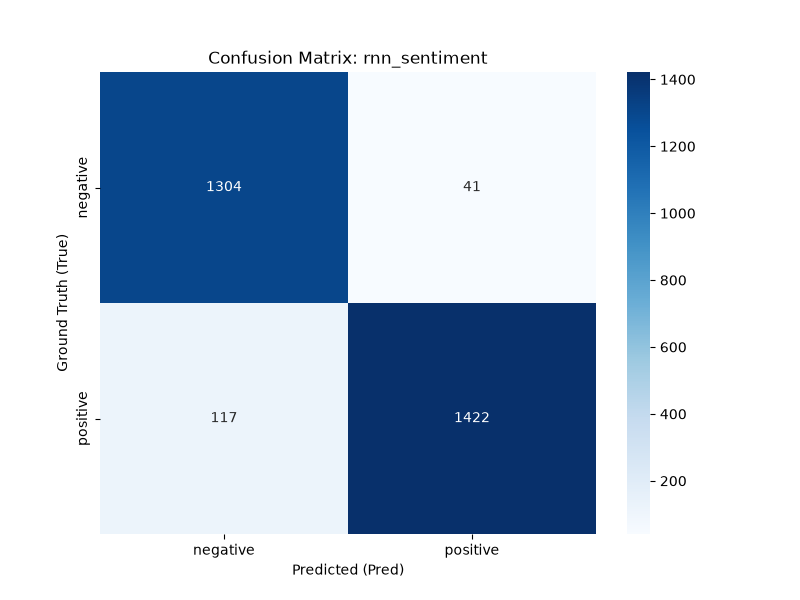
\includegraphics[width=\linewidth,height=0.68\textheight,keepaspectratio]{../images/rnn/rnn_sentiment_confusion_matrix.png}
    \end{column}
    \begin{column}{0.48\textwidth}
      \centering
      {\small\textbf{BidirLSTM} — Acc: 0.94, F1: 0.94}\\[0.3em]
      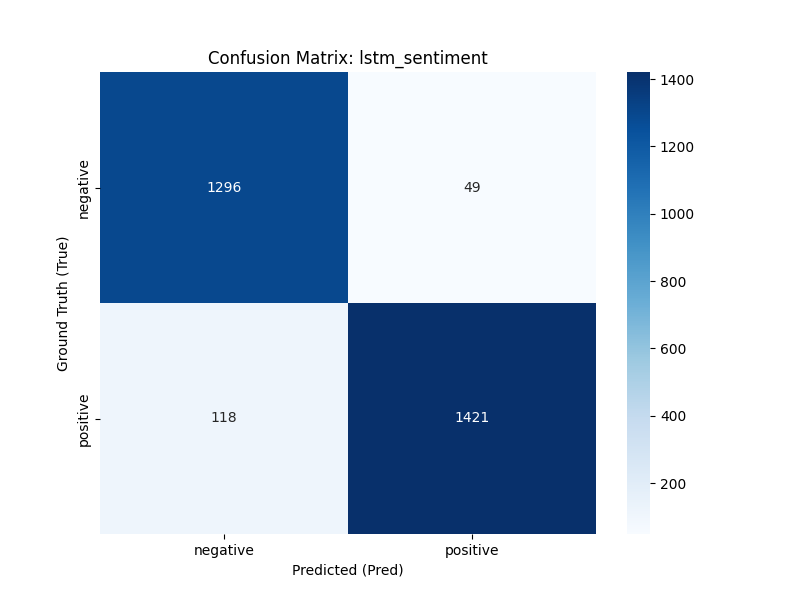
\includegraphics[width=\linewidth,height=0.68\textheight,keepaspectratio]{../images/lstm/lstm_sentiment_confusion_matrix.png}
    \end{column}
  \end{columns}
\end{frame}

% ==============================================================================
% SLIDE 12: Sentiment Confusion Matrix (Transformer) & Error Analysis
% ==============================================================================
\begin{frame}{Error Analysis: Sentiment Confusion Matrices (2/2)}
  \framesubtitle{Test set ($N = 2,884$) — \texttt{MultiTaskTransformer} \& cross-model comparison}
  \begin{columns}[c,totalwidth=\textwidth]
    \begin{column}{0.52\textwidth}
      \centering
      {\small\textbf{MultiTaskTransformer} — Acc: 0.93, F1: 0.93}\\[0.3em]
      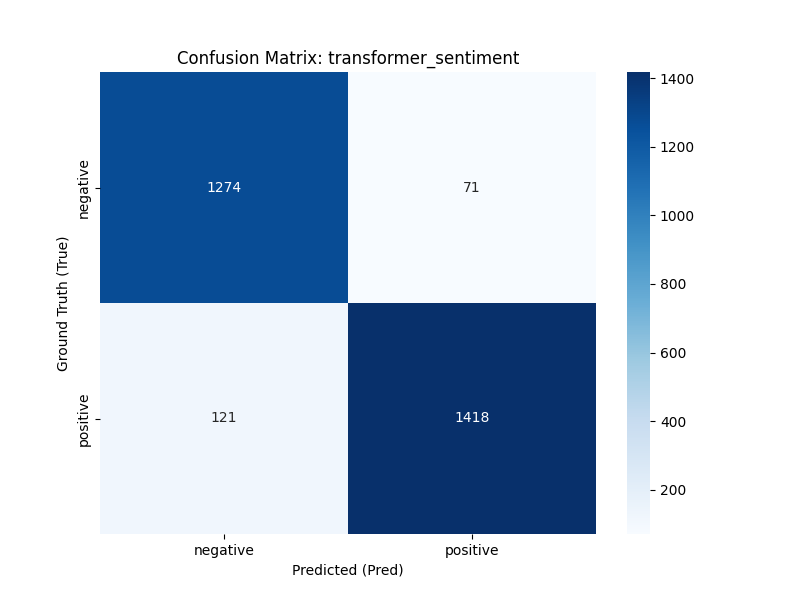
\includegraphics[width=\linewidth,height=0.68\textheight,keepaspectratio]{../images/transformer/transformer_sentiment_confusion_matrix.png}
    \end{column}
    \begin{column}{0.45\textwidth}
      \textbf{Sentiment Error Analysis}
      \begin{itemize}
        \item \textbf{High negative recall ($0.95$--$0.97$):} BiGRU misclassifies only $41$ negative samples ($3.0\%$), vs. $49$ for BiLSTM and $71$ for Transformer.
        \item \textbf{Dominant error mode:} Positive reviews misclassified as negative ($117$--$121$ cases across all models), typically constructive feedback containing negation words.
        \item \textbf{Recurrent advantage:} Sequence order modeling in BiGRU/BiLSTM handles negation scope better than from-scratch self-attention.
      \end{itemize}
    \end{column}
  \end{columns}
\end{frame}

% ==============================================================================
% SLIDE 13: Topic Confusion Matrices (BiGRU & BiLSTM)
% ==============================================================================
\begin{frame}{Error Analysis: Topic Confusion Matrices (1/2)}
  \framesubtitle{Test set ($N = 2,884$) — \texttt{BidirRNN} (BiGRU) vs. \texttt{BidirLSTM}}
  \begin{columns}[c,totalwidth=\textwidth]
    \begin{column}{0.48\textwidth}
      \centering
      {\small\textbf{BidirRNN (BiGRU)} — Acc: 0.91, F1: 0.88}\\[0.3em]
      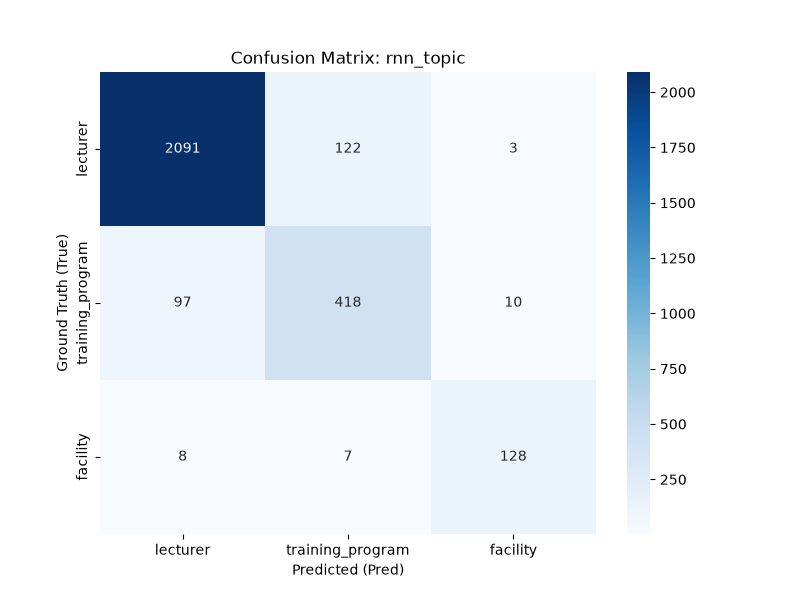
\includegraphics[width=\linewidth,height=0.68\textheight,keepaspectratio]{../images/rnn/rnn_topic_confusion_matrix.png}
    \end{column}
    \begin{column}{0.48\textwidth}
      \centering
      {\small\textbf{BidirLSTM} — Acc: 0.91, F1: 0.87}\\[0.3em]
      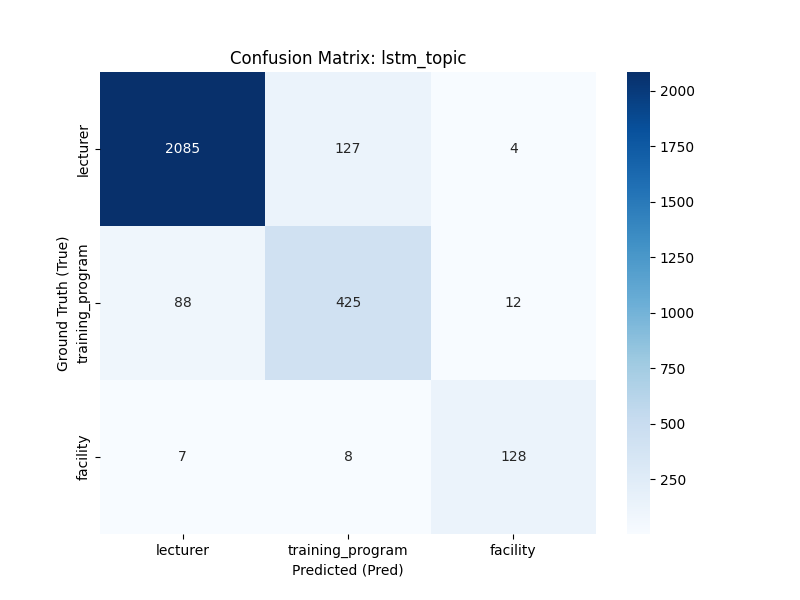
\includegraphics[width=\linewidth,height=0.68\textheight,keepaspectratio]{../images/lstm/lstm_topic_confusion_matrix.png}
    \end{column}
  \end{columns}
\end{frame}

% ==============================================================================
% SLIDE 14: Topic Confusion Matrix (Transformer) & Error Analysis
% ==============================================================================
\begin{frame}{Error Analysis: Topic Confusion Matrices (2/2)}
  \framesubtitle{Test set ($N = 2,884$) — \texttt{MultiTaskTransformer} \& cross-model comparison}
  \begin{columns}[c,totalwidth=\textwidth]
    \begin{column}{0.52\textwidth}
      \centering
      {\small\textbf{MultiTaskTransformer} — Acc: 0.91, F1: 0.86}\\[0.3em]
      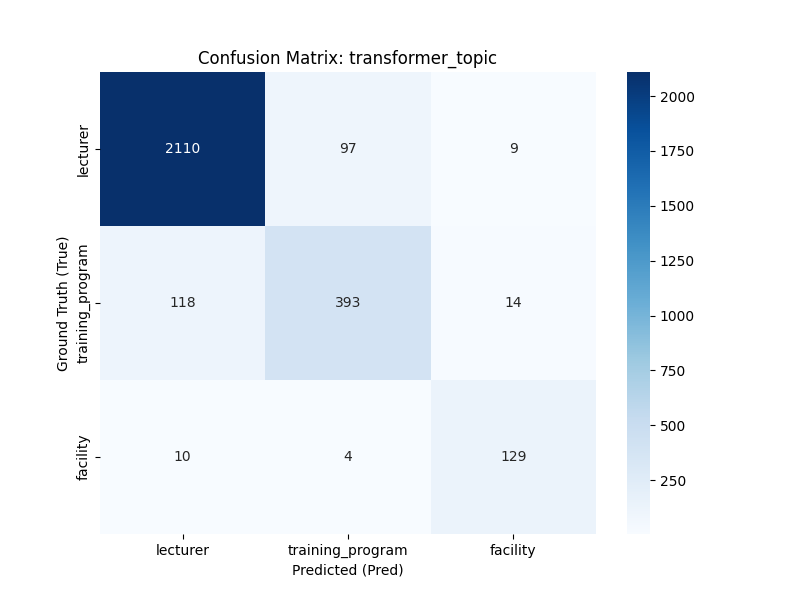
\includegraphics[width=\linewidth,height=0.68\textheight,keepaspectratio]{../images/transformer/transformer_topic_confusion_matrix.png}
    \end{column}
    \begin{column}{0.45\textwidth}
      \textbf{Topic Error Analysis}
      \begin{itemize}
        \item \textbf{\texttt{lecturer} ($0.95$ F1):} Dominant class ($76.8\%$) is cleanly separated across all three backbones.
        \item \textbf{\texttt{training\_program} ($0.77$--$0.78$ F1):} Most errors confuse \texttt{training\_program} with \texttt{lecturer} ($97$--$118$ cases), since curriculum comments often mention the instructor.
        \item \textbf{\texttt{facility} ($0.87$--$0.90$ F1):} Despite only $143$ test samples ($5.0\%$), distinct keywords (room, projector, wifi) yield high accuracy.
      \end{itemize}
    \end{column}
  \end{columns}
\end{frame}

% ==============================================================================
% SLIDE 13: Key Takeaways & Future Work
% ==============================================================================
\begin{frame}{Key Takeaways \& Future Work}
  \framesubtitle{Summary of empirical findings and next engineering steps}
  \begin{columns}[T,totalwidth=\textwidth]
    \begin{column}{0.48\textwidth}
      \textbf{Key Findings}
      \begin{itemize}
        \item \textbf{Inductive bias matters on 10k samples:} Recurrent models (BiGRU, BiLSTM) outperform a from-scratch Transformer on short Vietnamese feedback.
        \item \textbf{Right-sized capacity wins:} Compact BiGRU ($h=96$) generalizes better than BiLSTM ($h=256$) with $6.5\times$ smaller model size.
        \item \textbf{Fair multi-task comparison:} Aligning RNN loss weights to $(1.0, 1.0)$ confirms BiGRU's lead is architectural, not loss-weighting bias.
      \end{itemize}
    \end{column}
    \begin{column}{0.48\textwidth}
      \textbf{Future Improvements}
      \begin{itemize}
        \item \textbf{Pretrained Vietnamese encoders:} Replace whitespace tokenization with PhoBERT or ViDeBERTa.
        \item \textbf{Imbalance-aware training:} Use class weights or focal loss for \texttt{training\_program}.
        \item \textbf{Codebase unification:} Consolidate \texttt{lstm\_pip.py}, \texttt{rnn\_pip.py}, and \texttt{transformer\_pip.py} into one shared trainer.
      \end{itemize}
    \end{column}
  \end{columns}
\end{frame}

\end{document}
